\chapter{Números (3º Bimestre)}

\section{Probabilidades}

We already saw elementary concept of probability in the 4º bimestre of the
8ª série do Ensino Fundamental. A probabilidade é a
característica de um evento, que faz com que existam razões para criar que este
se realizará. A probabilidade $p$ de que ocorra um evento $S$ em um total de
$n$ casos possívels igualmente prováveis é igual a razão entre o número de
ocorrências $h$ do evento $S$ (casos favoráveis) e o número total de casos
possíveis $n$: $p=P\left(S\right)=\frac {h}{n}$.

Se $A$ e $B$ são dois eventos mutuamente exclusivos, temos
$P(A \text{ou} B) = P(A) + P(B)$. Se $A$ e $B$ são não exclusivos,
$P(A \text{e} B) \neq 0$ e
$P(A \text{ou} B) = P(A) + P(B) - P(A \text{e} B)$.
Se $A$ e $B$ são independentes,
${P(A \text{e} B)} = {P(A)} \times {P(B)}$
Se $A$ e $B$ são dependentes, e $P\left(B/A\right)$ é a probabilidade
de $B$ sabendo que $A$ ocorre, temos
${P(A \text{e} B)} = {P(A)} \times {P\left(B/A\right)}$.

\subsection*{Exercício 1}

We suppose that we have a bag with $10$ balls numeroted from $1$ and $10$.

\begin{enumerate}
\item If we pick a random ball from the bag. What is the probability it has
  number $5$?
\item What is the probability that the ball number is $\geq 7$.
\item What is the probability that the ball number is $\geq 7$ or
  that it has number $5$?
\item If we pick one ball put it back into the bag and pick a ball again,
  what is the probability that the first ball is $5$ and the second is $\geq 7$?
\item What is the probability that the first ball is $5$ or that the second
  is $\geq 7$?
\item
  If instead we do not put the first ball back before picking a second ball,
  what is the probability that the first ball is $5$ and the second is
  $\geq 7$?
\end{enumerate}

\section{Arranjos, combinações e permutações}

In the previous bimestre, we mention the concept of permutações on a set of
$n$ objects as the act of ordering them.
To do that, we pick the first object among the $n$ elements, the
second object among $n-1$ remaining elements, the third object among the $n-2$
remaining elements, ..., the $n-1$-th object among the $2$ remaining elements
and finally the $n$-th is remaining element. This gives
$1 \times 2 \times 3 \dots n = n!$ possible permutations.

If we only pick a subset of $k < n$ elementos to do the ordering, then
we obtain
$A_k^n = n \times {(n-1)} \times \dots {(n - k + 1)} = \frac{n!}{{(n-k)}!}$
possibilities. These are called arranjos de $n$ elementos tomados $k$ a $k$.

Combinações of $k$ elementos among $n$ are the ways to pick a subset of $k$
objects from a set of $n$ objects. This is the same as arranjos but we disregard
the order of the $k$ objects chosen. Since each of these subsets of $k$ elements
can be order in $k!$ many ways, the number of combinações is
$\binom{n}{k} = \frac{A_k^n}{k!} = \frac{n!}{k! {(n-k)}!}$.

\subsection*{Exercício 2}

\begin{enumerate}
\item List all the permutations of the set
  $\{\text{A}, \text{B}, \text{C}\}$. How many are there?
\item List all the arranjos of the set
  $\{\text{A}, \text{B}, \text{C}, \text{D}\}$ tomados $2$ a $2$.
  How many are there?
\item List all the combinações of the set
  $\{\text{A}, \text{B}, \text{C}, \text{D}, \text{E}\}$ tomados $2$ a $2$.
  How many are there?
\end{enumerate}

\subsection*{Exercício 3}
\begin{enumerate}
\item List the words of two letters that we write with the alphabet
  $\{\text{A}, \text{B}\}$? How many are there?
\item
  We suppose that we place the elements of the sets
  $\{\text{A}, \text{B}, \text{C}, \text{D}\}$
  on a uma circunferência de círculo (the angular coordinate of letters and
  orientation of the circle does not matter). How many different ways
  are there to do that?
\item We suppose that we have three letters $\text{A}$ and
  two letters $\text{B}$.
  List the words of $5$ letters that we can write with them.
\item How many ways are there to write words of $6$ letters using
  three letters $\text{A}$, two letters $\text{B}$ and one letter
  $\text{C}$?
\item How many words of two letters can we write with the alphabet
  $\{\text{A}, \text{B}, \text{C}, \text{D}\}$.
  We now suppose that we do not distinguish anagrams
  (words using the same letters in a different order) that is
  AB and BA are the same. How many elements are there? List them.
\end{enumerate}

\subsection*{Exercício 4 (triângulo de Pascal)}

\begin{enumerate}

\item What is the unique way to choose $n$ elements from a set of $n$ elements?
  Deduce the value of $\binom{n}{n}$.

\item We suppose $n > 0$. How many ways are there to choose one element from
  a set of $n$ elements? Deduce the value of $\binom{n}{1}$.

\item Let $n \geq 0$ and $0 \leq k \leq n$.
  In order to choose $n - k$ elements, we can equivalently choose the $k$
  elements to discard. Deduce the value of $\binom{n}{n - k}$.

\item Let $0 < k < n$. Suppose a set containing $n$ elements and fix
  $x$ one of these elements. Determine the number of ways to choose $k$ of
  these elements by distinguishing the cases where $x$ is chosen or not.
  Deduce the value of $\binom{n-1}{k-1} + \binom{n-1}{k}$.

\item We construct the triângulo de Pascal as follows:
  for any $n \geq 0$, the $n+1$-th row has $n+1$ elements given by
  $\binom{n}{0}, \binom{n}{1}, \binom{n}{2}, \dots, \binom{n}{n-1},
  \binom{n}{n}$.
  Draw the first rows ($n \leq 5$) of the triangle, horizontally centering them.

\item Explain how the previous formulas are interpreted visually on the
  triângulo de Pascal.

\end{enumerate}

\section{Distribuição binomial de probabilidades}

We already mentioned Distribuição binomial de probabilidades in an exercise
the 4º bimestre of the 8ª série do Ensino Fundamental. We consider an experiment
with probability of success $p$ and (thus) of probability of failure $q=1-p$.
We repeat this experiment $n$ times and for any $1 \leq i \leq n$ we note
$A_i$ the event saying that the $i$-th succeeded and assume that all these
events are independent from each other. Then we still have
$P(A_i) = p$ and $P(\bar{A_i}) = q$.

We now pick $k$ steps
$1 \leq i_1 < i_2 < \dots < i_k \leq n$ and denote $B_{i_1, i_2, \dots, i_k}$ the
probability that the experiment succeeds at these step $i_1,i_2, \dots, i_k$
and fails at the other steps. $P(B_{i_1, i_2, \dots, i_k})$ is thus
of the probability that the expected event happens at step $1 \leq i \leq n$
($P(A_i)=p$ if $i$ is one these $i_j$'s and $P(\bar{A_i})=q$ otherwise) that is
$p^k q^{n-k}$.

Finally, for any $0 \leq k \leq n$ we can $C_k$ the events saying that the
experiment succeeds a $k$ steps and thus fails the $n-k$ other steps.
Since the events $B_{i_1, i_2, \dots, i_k}$ are pairwise exclusive by definition,
$P(C_k)$ is the sum of the $P(B_{i_1, i_2, \dots, i_k})$'s for all possible choices
of $k$ elements among $n$. Hence $P(C_k) = \binom{n}{k} p^k q^{n-k}$.
The events $C_k$ are pairwise exclusive by definition. Moreover, since we
necessarily have exactly $k$ successes for some $0 \leq k \leq n$
these probabilities sum up to
$$1 = \sum_{0 \leq k \leq n} \binom{n}{k} p^k q^{n-k}$$.

\subsection*{Exercício 5 (binômio de Newton)}

Let $x, y \in \mathbb R$ and $n \geq 1$ an integer number.
We wish to expand ${(x+y)}^n = {(x+y)}{(x+y)}{(x+y)}\dots{(x+y)}$.
Recall that this is the sum of the terms, where each term is obtained as
follows: in each of the $n$ factors $(x+y)$ we pick either a $x$ or a $y$ then
take the product of the $n$ variables chosen.

\begin{enumerate}
\item Determine the expansion for $n = 1, 2, 3$. Compare with the triângulo de
  Pascal.
\item Let $0 \leq k \leq n$. We pick $1 \leq i_1 < i_2 < \dots < i_k$ indices.
  What is the term obtain by choosing a $x$ for the $i_1$-th,
  $i_2$-th, .., $i_k$-th factors and a $y$ for the other factors.
  How many ways are there to obtain this term?
\item Deduce the expansion of ${(x+y)}^n$.
\item Compare with the binomial distribution where $x=p$ and $y=q$.
\end{enumerate}

\subsection*{Exercício 6}

We repeat the game ``cara'' ou ``coroa'' $n$ vezes.

\begin{enumerate}
\item What is the probability to win the game at the first attempt?
\item If $n=3$, what is the probability to win the game for all the attempts?
\item For $0 \leq k \leq n$,
  what is probability to win exactly $k$ attempts over $n$?
\item Express the number of possible results
  ``cara''/``coroa'' in function of $n$.
\item For $0 \leq k \leq n$, indicate the number of results corresponding to
  exactly $k$ successes.
\end{enumerate}

\subsection*{Exercício 7}

We consider a bag containing $3$ red balls, $2$ blue balls and $4$ green balls.

\begin{enumerate}
\item We pick one random ball.
  What are the probabilities to pick a red, blue, and red
  ball?
\item We pick a second random ball.
  What is the probability that it is red, assuming
  that the first one was red?
\item What is the probability that the two balls are red?
\item More generally, what is the probability $p$ that the two balls have same
  colors?
\item Deduce the probability $q$ to pick two balls of distinct colors.
\item We put back the balls into the bag and pick two random balls again.
  What is the probability that we obtain two balls of same colors
  in one case and two balls of distinct colors in another case?
\item Suppose that we actually repeat the experiments $5$ times.
  What is the probability that we obtain two balls of same colors
  in two cases and two balls of distinct colors in the three other cases?
\end{enumerate}

\section{Solução do Exercícios}

\subsection*{Exercício 1}

\begin{enumerate}
\item There are $10$ possibilities and in only one case the ball has number $5$
  so the probability is $\frac{1}{10}$.
\item There are now $4$ casos favoráveis ($7,8,9,10$) so
  so the probability is $\frac{4}{10} = \frac{2}{5}$.
\item The two events são exclusivos so
  the probability is $\frac{1}{10} + \frac{2}{5} = \frac{1}{2}$.
  Alternatively, these correspond to $5$ casos favoráveis
  ($5,7,8,9,10$) so again the probability is $\frac{5}{10} = \frac{1}{2}$.
\item The two events são independentes,
  so the probability is $\frac{1}{10} \frac{2}{5} = \frac{1}{25}$.
\item The two events não são exclusivos so the probability is
  $\frac{1}{10} + \frac{2}{5} - \frac{1}{25} = \frac{23}{50}$
\item The two events são dependentes. The probability that the first ball is
  $5$ is still $\frac{1}{10}$. However, the probability that first ball
  is $\geq 7$ knowing that we removed the $5$ is now $\frac{4}{9}$.
  So the probability of the event is $\frac{1}{10} \frac{4}{9} = \frac{2}{45}$.
\end{enumerate}

\subsection*{Exercício 2}

\begin{enumerate}
\item ABC, ACB, BAC, BCA, CAB, CBA. There are $3! = 6$ such permutations.
\item AB, AC, AD, BA, BC, BD, CA, CB, CD, DA, DB, DC.
  There are $\frac{4!}{{(4-2)}!} = \frac{24}{2} = 12$ such arranjos.
\item AB, AC, AD, AE, BC, BD, BE, CD, CE, DE.
  There are $\frac{5!}{{2!}{(5-2)}!} = \frac{120}{2 \times 6} = 10$
  such combinações.
\end{enumerate}

\subsection*{Exercício 3}
\begin{enumerate}
\item AA, AB, AC, BA, BB, BC, CA, CB, CC.
  There are $3$ possibilities for the first letter and
  $3$ possibilities for the second letter so there are $3^2 = 9$ such words.
  Alternatively, there are $3!=6$ permutations plus $3$ cases where we repeat
  two letters (AA, BB, CC).
\item This is the number of permutations without distinguish which is the first
  letter. So there are $\frac{4!}{4} = 6$ ways: ABCD,ABDC,ACBD,ACDB,ADBC,ADCB.
\begin{center}
  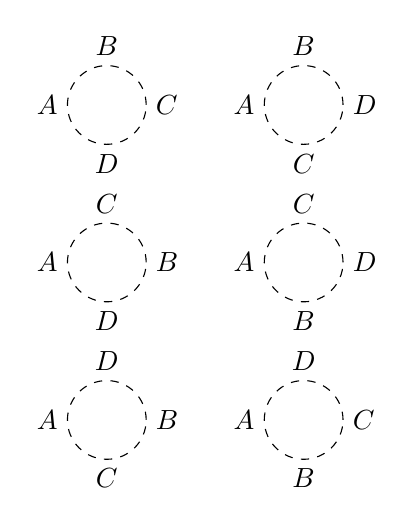
\begin{tikzpicture}[scale=.5]
    \begin{scope}[shift={(0,0)}]
    \draw[style=dashed] (0,0) circle(1);
    \draw (-1, 0) node[left] {$A$}
          (0,  1) node[above]{$B$}
          ( 1, 0) node[right]{$C$}
          (0, -1) node[below]{$D$};
    \end{scope}
    \begin{scope}[shift={(5,0)}]
    \draw[style=dashed] (0,0) circle(1);
    \draw (-1, 0) node[left] {$A$}
          (0,  1) node[above]{$B$}
          ( 1, 0) node[right]{$D$}
          (0, -1) node[below]{$C$};
    \end{scope}
    \begin{scope}[shift={(0,-4)}]
    \draw[style=dashed] (0,0) circle(1);
    \draw (-1, 0) node[left] {$A$}
          (0,  1) node[above]{$C$}
          ( 1, 0) node[right]{$B$}
          (0, -1) node[below]{$D$};
    \end{scope}
    \begin{scope}[shift={(5,-4)}]
    \draw[style=dashed] (0,0) circle(1);
    \draw (-1, 0) node[left] {$A$}
          (0,  1) node[above]{$C$}
          ( 1, 0) node[right]{$D$}
          (0, -1) node[below]{$B$};
    \end{scope}
    \begin{scope}[shift={(0,-8)}]
    \draw[style=dashed] (0,0) circle(1);
    \draw (-1, 0) node[left] {$A$}
          (0,  1) node[above]{$D$}
          ( 1, 0) node[right]{$B$}
          (0, -1) node[below]{$C$};
    \end{scope}
    \begin{scope}[shift={(5,-8)}]
    \draw[style=dashed] (0,0) circle(1);
    \draw (-1, 0) node[left] {$A$}
          (0,  1) node[above]{$D$}
          ( 1, 0) node[right]{$C$}
          (0, -1) node[below]{$B$};
    \end{scope}
  \end{tikzpicture}
\end{center}
\item
  To write a word, we need to choose $3$ positions to put the letters A and we
  put the letters B in the remaining positions. So
  there are $\binom{5}{3} = 10$ possibilities:
  AAABB, AABAB, AABBA, ABAAB, ABABA, ABBAA, BAAAB, BAABA, BABAA, BBAAA.
\item
  We choose $3$ positions among the $6$ available
  for the letters $A$, which gives $\binom{6}{3}$ possibilities.
  We choose $2$ positions for the letters $B$ among the three remaining
  positions, which gives $\binom{3}{2}$ possibilities. Finally, we put the
  $C$ at the last position. This gives a total of
  $\binom{6}{3} \times \binom{3}{2} = 20 \times 3 = 60$ words.
\item There are $4$ possibilities for the first letter and
  $4$ possibilities for the second letter, so there are $4^2=16$ words.
  If we do not distinguish anagrams, these are
  AA, AB, AC, AD, BB, BC, BD, CC, CD, DD. This is the same as choosing
  $2$ elements from the set
  $\{\text{A}, \text{B}, \text{C}, \text{D}, \text{*} \}$
  where $\text{*}$ combined with a letter represents a word with this letter
  repeated twice. So there are indeed $\binom{5}{2} = 10$ cases.
\end{enumerate}

\subsection*{Exercício 4 (triângulo de Pascal)}

\begin{enumerate}
  \item Only one way: choose them all! So $\binom{n}{n} = 1$.
  \item There are $n$ choices possible (one for each element) so
    $\binom{n}{1} = n$.

  \item $\binom{n}{n - k} = \binom{n}{k}$, since the left hand side is the
    way to choose $n - k$ elements and the right hand side the way to choose
    $k$ elements to discard.

  \item If we require that $x$ is chosen, then it remains to choose $k-1$
    elements from the $n-1$ other elements that is
    $\binom{n-1}{k-1}$ possibilities.
    If we require that $x$ is not chosen, then we must
    choose $k$ elements from the $n-1$ other elements, that is
    $\binom{n-1}{k}$ possibilities.
    If we sum up all these possibilities we obtain the number of ways to choose
    $k$ elements among $n$, that is
    $\binom{n}{k} = \binom{n-1}{k-1} + \binom{n-1}{k}$

  \item We find the following schema:
    \begin{center}
      \begin{tikzpicture}[yscale=-1]
        \draw
        (0, 0) node {$1$}
        (-.5, 1) node {$1$} (.5, 1) node {$1$}
        (-1, 2) node {$1$} (0, 2) node {$2$} (1, 2) node {$1$}
        (-1.5, 3) node {$1$} (-.5, 3) node {$3$} (.5, 3) node {$3$} (1.5, 3) node {$1$}
        (-2, 4) node {$1$} (-1, 4) node {$4$} (0, 4) node {$6$} (1, 4) node {$4$} (2, 4) node {$1$}
        (-2.5, 5) node {$1$} (-1.5, 5) node {$5$} (-.5, 5) node {$10$} (.5, 5) node {$10$} (1.5, 5) node {$5$} (2.5, 5) node {$1$}
        ;
      \end{tikzpicture}
    \end{center}

\item $\binom{n}{n} = 1$ says that the last element of each row is a $1$.
  $\binom{n}{1} = n$ for $n > 0$ says that the second element of the
  $n+1$-th row is $n$. $\binom{n}{n - k} = \binom{n}{k}$ explains the symmetry
  of the triangle with respect to the central vertical axis.
  Finally, $\binom{n}{k} = \binom{n-1}{k-1} + \binom{n-1}{k}$ says that to
  obtain the element $\binom{n}{k}$ of the $n+1$-th row, we sum up the two
  elements above it (for example $3=1+2$ or $10 = 4+6$). This gives a recursive
  way to build the triângulo de Pascal.

\end{enumerate}

\subsection*{Exercício 5 (binômio de Newton)}

\begin{enumerate}
\item $${(x+y)}^1 = x + y$$
  $${(x+y)}^2 = x^2 + 2xy + y^2$$
  $${(x+y)}^3 = {(x^2 + 2xy + y^2)}{(x+y)} =
  x^3 + 2x^2y + xy^2 + x^2y + 2xy^2 + y^3 =
  x^3 + 3x^2y + 3xy^2 + y^3$$
The coefficients obtained $(1, 1)$, $(1, 2, 1)$ and $(1, 3, 3, 1)$ are the same
as in the triângulo de Pascal.

\item We obtain the term $x^k y^{n-k}$. There are $\binom{n}{k}$ ways to choose
  $k$ indices for $x$ among $n$ factors.

\item We obtain
  $${(x+y)}^n = \sum_{k=0}^n \binom{n}{k} x^k y^{n-k}$$

\item We have $x+y=p+q=1$ so we recover the expression saying that
  $1 = \sum_{k=0}^n P(C_k)$ where
  $P(C_k) = \binom{n}{k} x^k y^{n-k}$ is the probability to have exactly
  $k$ success.
\end{enumerate}

\subsection*{Exercício 6}

\begin{enumerate}
\item $\frac{1}{2}$ (assuming the face of the coin are perfectly symmetric)
\item $\frac{1}{2} \times \frac{1}{2} \times \frac{1}{2} = \frac{1}{8} = 0.125$.
\item This is a binomial distribution with $p=q=\frac{1}{2}$.
  Hence if $A_k$ is the event ``exactly $k$ successes occur'' then
  $P(A_k) = \binom{n}{k} p^k q^{n-k} = \frac{1}{2^n} \binom{n}{k}$.
\item $2^n$
\item All the cases are equiprobable, so
  $P(A_k) = \frac{N_k}{2^n}$ where $N_k$ is the number of results corresponding
  to exactly $k$ successes. Hence $N_k = \binom{n}{k}$.
\end{enumerate}

\subsection*{Exercício 7}

\begin{enumerate}
\item We have $2+3+4=9$ balls. The probability to pick a red ball is
  $\frac{3}{9} = \frac{1}{3}$. The probability to pick a blue ball is
  $\frac{2}{9}$. The probability to pick a green ball is
  $\frac{4}{9}$.
\item If the first ball was red, then it remains $2$ red balls over the $8$
  remaining balls, so the probability is $\frac{2}{8}=\frac{1}{4}$.
\item $\frac{1}{3} \frac{1}{4} = \frac{1}{12}$
\item Similarly, the probability to pick two blue balls is
  $\frac{2}{9} \frac{1}{8} = \frac{1}{36}$ and
  the probability to pick two green balls is
  $\frac{4}{9} \frac{3}{8} = \frac{1}{6}$. The three events are pairwise
  exclusive, so the probability to pick two balls of same color
  is $\frac{1}{12} + \frac{1}{36} + \frac{1}{6} = \frac{5}{18}$.
\item $q = 1 - p = \frac{13}{18}$.
\item $pq + qp = 2pq = \frac{65}{162}$.
\item $\binom{5}{2} p^2 q^3 = 10p^2q^3 = \frac{274625}{944784}$.
\end{enumerate}
